\begin{center}
\section{PROPOSED METHODOLOGY}
\end{center}
\subsection{Software Development Life Cycle}
I have chosen the incremental model for the software development life cycle due to its unique advantages that align with the goals and complexities of the Student Access Portal (SAP) project.

The incremental model is an ideal fit for our project because it allows us to prioritize key features and deliver tangible results in smaller, manageable increments. Given the dynamic nature of educational technology, where user needs and requirements might evolve during development, the incremental approach enables us to adapt and respond more effectively to these changes.

With the SAP, we aim to deliver value to our users as early as possible. By breaking down the development process into incremental stages, we can release functional modules or subsets of the application in shorter time frames. This allows us to gather user feedback, address concerns, and incorporate improvements continuously, ensuring that the final product meets or exceeds user expectations.\\
\vspace{0.5in}
\begin{figure}[h]
    \centering
    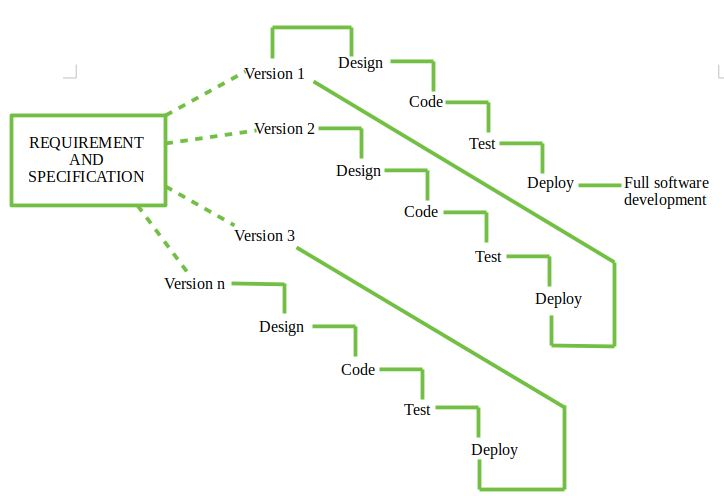
\includegraphics[width = 5in]{Proposal/static/incremental.png}
    \caption{Incremental Model}
    \label{fig:enter-label}
\end{figure}
\newpage

\begin{itemize}
    \item \textbf{Requirement Gathering:}\\
    Requirements for the System Administration Portal (SAP) project are gathered through a combination of user interviews, surveys, and consultations with students, instructors, and administrative staff.Regular feedback loops are established, enabling continuous adjustments based on evolving user expectations and emerging trends in educational technology.
    \item \textbf{Design:}\\
    The design phase of the Student Access Portal (SAP) project involves creating a detailed architectural blueprint and user interface (UI) design that aligns with the project's goals and user requirements. The structure of database is planned, use cases evaluated, user interface designed and security was integrated into the design.
    \item \textbf{Coding and Testing:}\\
    In the coding phase, we have decided to use the MERN stack.This phase involves writing clean, efficient code, integrating frontend and backend components, and implementing features. Concurrently, rigorous testing is conducted, including unit, integration, and user acceptance testing, ensuring the SAP's functionality, security, and performance align with requirements.
    \item \textbf{Deployment:}\\
    We will set up the deployment infrastructure the web application considering the cost effectiveness and efficiency. This involves setting up servers, and ensuring the platform's security measures. Once deployed, the SAP becomes accessible to users, and ongoing monitoring and maintenance processes begin to ensure optimal performance and user satisfaction.
\end{itemize}
\newpage
\subsection{System Development Tools}
\begin{itemize}
    \item \textbf{MongoDB:}\\
    MongoDB is utilized in the construction of the System Administration Portal (SAP) as the primary database management system. MongoDB, a NoSQL database, offers a flexible and scalable solution, aligning well with the dynamic requirements of the SAP. It allows us to store various types of data, including user profiles, resource metadata, room collaborations, and notifications, in a schema-less format, accommodating changes and additions without complex migrations.MongoDB's document-oriented model enables us to structure data in a way that mirrors real-world entities, such as students, instructors, courses, and resources. This enhances the efficiency of querying and retrieving data, making it well-suited for managing user profiles, room information, and resource associations. Additionally, MongoDB's support for indexing and aggregation pipelines ensures that data access remains performant as the platform scales.\cite{mongo}
    \item \textbf{ReactJS:}\\
    We preferred ReactJS as the frontend library to create dynamic, interactive user interfaces. It is preferrable due to it's benefits like: Component-based development, Efficient UI updates, Responsive Design, Ecosystem and Community, Third Party Integrations etc.\cite{node}
    \item \textbf{ExpressJS:}\\
     ExpressJS serves as the backbone of the SAP's backend, facilitating request handling, route management, middleware integration, and database interactions. Its versatility and efficiency make it an ideal choice for building a secure, responsive, and scalable backend system that complements the frontend, ensuring a cohesive and seamless user experience within the application. ExpressJS serves as the web server for the SAP, handling incoming HTTP requests, routing them to the appropriate endpoints, and responding with the required data.Express simplifies route handling, allowing us to define clear and structured routes for various API endpoints.Express middleware enables us to process requests before they reach the intended route, facilitating tasks such as authentication, data validation, error handling, and logging. This ensures a secure and efficient backend operation.Express simplifies the creation of robust APIs, making it efficient to expose functionalities to the frontend (built with ReactJS) and other components of the application.\cite{express}
    \item \textbf{NodeJS:}\\
    Node.js serves as the backbone that powers the SAP's responsiveness, scalability, and real-time capabilities. Its single language approach, non-blocking architecture, and extensive ecosystem make it an ideal choice for creating a modern, efficient, and highly interactive educational platform that serves both students and instructors effectively. Node.js enables the use of JavaScript on both the client and server sides, ensuring consistency and reducing the need for context-switching between languages.  Node.js employs a non-blocking, event-driven architecture, making it highly efficient in handling asynchronous tasks.Node.js is known for its ability to handle a large number of concurrent connections with minimal resource usage.Node.js is well-suited for building microservices and RESTful APIs, aligning with the architecture of the SAP. Node.js's event-driven nature makes it an excellent choice for real-time applications.\cite{node}
    \item \textbf{GitLab:}\\
    GitLab is selected for the development of the SAP due to its robust version control, code collaboration features, CI/CD capabilities, project management tools, and options for self-hosting. These aspects make GitLab a comprehensive platform that enhances the efficiency, security, and collaboration of the development process, aligning well with the goals of the SAP project.As for choosing GitLab over GitHub, there are several factors to consider. GitLab offers a more comprehensive feature set in its free plan, including built-in CI/CD pipelines and project management tools. This is advantageous for a project like the SAP, where an integrated development environment is crucial. Additionally, GitLab's self-hosting option provides us with greater control over our repositories, which can be essential for data privacy compliance.\cite{gitlab}
\end{itemize}
\newpage